% !TeIX spellcheck = cs_CZ
%{\tikzset{external/prefix={tikz/FYZII/}}
% \tikzset{external/figure name/.add={ch09_}{}}
%---------------------------------------------------------------------------------------------------
% file fey2ch09.tex
%---------------------------------------------------------------------------------------------------
%=========================== Kapitola: Elektřina v atmosféře =======================================
\setchaptertoc
\chapter{Elektřina v atmosféře}\label{fyz:IIchapIX}  
  \section{Gradient elektrického potenciálu v atmosféře}\label{fyz:IIchapIXsecI}  
    Za obyčejného dne nad rovinatou pouští nebo nad mořem vzrůstá elektrický potenciál asi o
    \num{100} voltů na metr vzhůru od zemského povrchu. Ve vzduchu tedy existuje vertikální
    elektrické pole \(E\) s velikostí \SI{100}{\V\per\m}. Směr pole je takový, jako kdyby zemský
    povrch měl záporný náboj. To znamená, že venku je potenciál ve výšce nosu o \num{200} voltů
    vyšší než potenciál na úrovni našich chodidel. Mohli bychom se zeptat: „Proč tedy neupevníme ve
    vzduchu ve vzdálenosti jeden metr od sebe dvě elektrody a nevyužijeme těch \num{100} voltů k
    napájení elektrického osvětlení?“ Nebo bychom se mohli podivit: Je-li mezi mým nosem a chodidly
    skutečně napětí 200 voltů, proč když vycházím z budovy, nedostanu elektrický šok?“

    Objasníme nejprve druhou otázku. Naše tělo je poměrně dobrým vodičem. Dotýkáme-li se země, spolu
    s ní vytváříte jednu ekvipotenciální hladinu. Ekvipotenciální hladiny jsou normálně rovnoběžné
    se zemským povrchem (obr. \ref{fyz:fig689a}), ale když je tam naše tělo, poruší se a pole vypadá
    asi tak, jako ukazuje obr. \ref{fyz:fig689b}. Mezi naší hlavou a chodidly je tedy téměř nulové
    napětí. Ze země přechází do naší hlavy náboje a pole se mění.

    \begin{figure}[ht!]
      \centering
      \subcaptionbox{\label{fyz:fig689a}}{\luafigure[0.8]{fyz_fig689a.pdf}}               \newline
      \subcaptionbox{\label{fyz:fig689b}}{\luafigure[0.8]{fyz_fig689b.pdf}}
      \caption{a) rozdělení potenciálu nad zemí. b) rozdělení potenciálu v blízkosti člověka 
               stojícího na otevřeném rovinném prostranství (\cite[s.~748]{Feynman02})}
      \label{fyz:fig689}
    \end{figure}

    Některé z těchto nábojů mohou být neutralizovány ionty ve vzduchu, jejich proud je však velmi
    malý, neboť vzduch je špatným vodičem.

    Jak můžeme měřit takové pole, změní-li se, když do něj něco vložíme? Existuje několik způsobů.
    Jeden způsob je umístit izolovaný vodič do určité vzdálenosti nad zemí a nechat jej tam, dokud
    nebude na stejném potenciálu jako vzduch. Necháme-li jej tam dostatečně dlouho, budou i při malé
    vodivosti vzduchu náboje z (nebo do) vodiče unikat, dokud se jeho potenciál nevyrovná s
    potenciálem vzduchu na stejné úrovni. Pak jej můžeme opět spustit k zemi a změřit změnu
    potenciálu. Rychlejší způsob je použít jako vodič vědro vody s malou dírkou. Vykapávající voda
    odnese přebytečné náboje a vědro bude mít tentýž potenciál jako vzduch. (Jak víme, náboje se
    zdržují na povrchu a odkapáváním kapek se „kousky povrchu“ odlamují.) Potenciál vědra je možné
    změřit elektrometrem.

    \begin{figure}[ht!]
      \centering
      \subcaptionbox{\label{fyz:fig690a}}{\luafigure[0.9]{fyz_fig690a.pdf}}               \newline
      \subcaptionbox{\label{fyz:fig690b}}{\luafigure[0.9]{fyz_fig690b.pdf}}
      \caption{a) Uzemněná kovová deska bude mít stejný plošný náboj jako zemský povrch.
               b) Když se deska přikryje uzemněným vodičem, nebude mít žádný plošný náboj.
               (\cite[s.~707]{Feynman02})}
      \label{fyz:fig690}
    \end{figure}

    Existuje ještě jeden způsob přímého měření \emph{gradientu} potenciálu. Protože existuje
    elektrické pole, má Země svůj povrchový náboj \((σ=ϵ_0E)\). Umístíme-li do blízkosti zemského
    povrchu rovnou kovovou desku \(A\) a uzemníme ji, objeví se na ní záporné náboje (obr.
    \ref{fyz:fig690a}). Přikryjeme-li tuto deskujinou uzemněnou vodivou deskou \(B\), objeví se
    náboje na ní a z původní desky \(A\) vymizí. Když odměříme náboj, jenž prochází z desky \(A\) k
    zemi (například galvanometrem připojeným k uzemňovacímu vodiči při jejím zakrývání, můžeme
    zjistit povrchovou hustotu náboje, která na něm byla, a tím zjistit i elektrické pole.

    Když jsme si připomněli, jak je možné elektrické pole v atmosféře měřit, budeme nyní pokračovat
    v jeho popisu. Měření především ukazují, že při výstupu do velkých výšek pole sice existuje, ale
    slábne. Zhruba po padesáti kilometrech je už velmi malé, takže většina změny potenciálu
    (integrál intenzity \(E\)) připadá na menší výšky. Celkový rozdíl potenciálu od povrchu Země k
    horní hranici atmosféry je asi \num{400000} voltů.

  \section{Elektrické proudy v atmosféře}\label{fyz:IIchapIXsecII}   
    Kromě gradientu potenciálu můžeme v atmosféře měřit také proud. Hustota proudu je malá - každým
    metrem čtverečním rovnoběžným se zemským povrchem prochází asi \num{10} pikoampérů. Vzduch
    zřejmě není dokonalý izolant a v důsledku jeho vodivosti prochází od oblohy dolů k zemi malý
    proud, vyvolaný právě popisovaným elektrickým polem.

    \begin{figure}[ht!] %\ref{fyz:fig691}
      \centering
      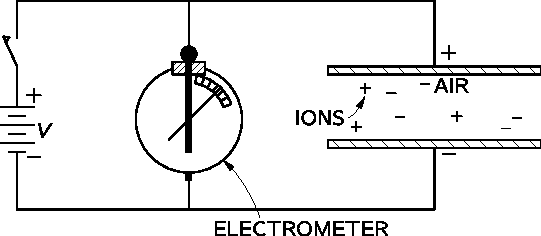
\includegraphics[width=0.8\linewidth]{fyz_fig691.pdf}
      \caption{Měření vodivosti vzduchu způsobené pohybem iontů
               (\cite[s.~707]{Feynman02})}
      \label{fyz:fig691}
    \end{figure}

    Proč je atmosféra vodivá? Mezi molekulami vzduchu se tu a tam vyskytne iont, řekněme molekula
    kyslíku, která přibrala jeden elektron navíc, nebo snad jeden elektron ztratila. Tyto ionty
    nezůstávají osamocené; svým elektrickým polem kolem sebe obvykle shromáždí několik dalších
    molekul. Každý iont se potom stává malou hrudkou, která je spolu s jinými podobnými hrudkami
    unášena polem, a při pomalém pohybu vzhůru nebo dolů vytváří pozorovatelný proud. Odkud ionty
    pocházejí? Nejdříve se lidé domnívali, že vznik iontů způsobuje radioaktivita Země. (Bylo známo,
    že záření z radioaktivních látek ionizuje molekuly ve vzduchu a tím jej dělá vodivým.) Částice,
    například \(\beta\)-záření, vyletují z atomových jader tak rychle, že vytrhávají elektrony z
    atomů a zanechávají za sebou ionty. Z této domněnky ovšem vyplývá, že při výstupu do větších
    výšek bychom našli menší ionizaci, protože všechna radioaktivita se nachází v Zemi - ve
    stopových množstvích radia, uranu, draslíku apod.

  \section{Původ atmosférických proudu}\label{fyz:IIchapIXsecIII}
  \section{Bouřky}\label{fyz:IIchapIXsecIV}
  \section{Mechanismus oddělování nábojů}\label{fyz:IIchapIXsecV}
  \section{Blesk}\label{fyz:IIchapIXsecVI}


    \begin{figure}[ht!] %\ref{fyz:fig692}
      \centering
      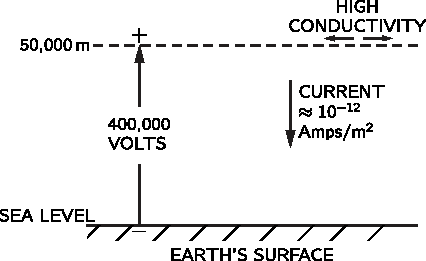
\includegraphics[width=0.6\linewidth]{fyz_fig692.pdf}
      \caption{
               (\cite[s.~707]{Feynman02})}
      \label{fyz:fig692}
    \end{figure}

    \begin{figure}[ht!] %\ref{fyz:fig693}
      \centering
      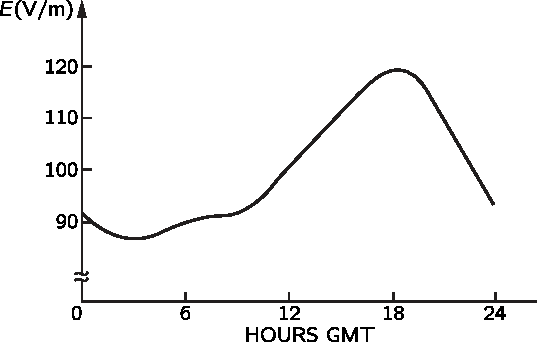
\includegraphics[width=0.6\linewidth]{fyz_fig693.pdf}
      \caption{
               (\cite[s.~707]{Feynman02})}
      \label{fyz:fig693}
    \end{figure}

    \begin{figure}[ht!] %\ref{fyz:fig694}
      \centering
      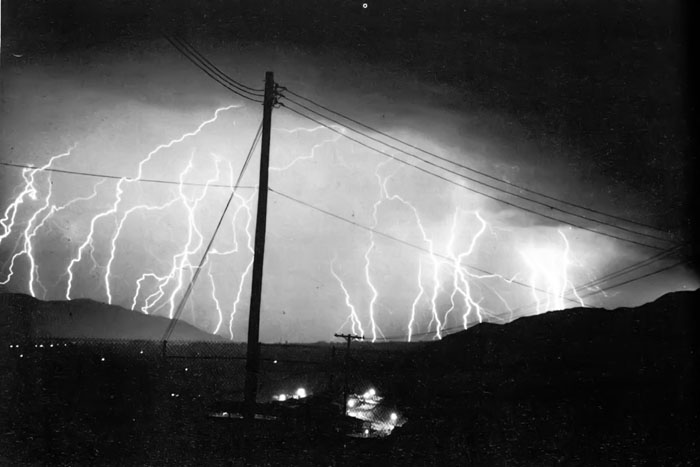
\includegraphics[width=0.6\linewidth]{fyz_fig694.jpg}
      \caption{
               (\cite[s.~707]{Feynman02})}
      \label{fyz:fig694}
    \end{figure}

    \begin{figure}[ht!] %\ref{fyz:fig695}
      \centering
      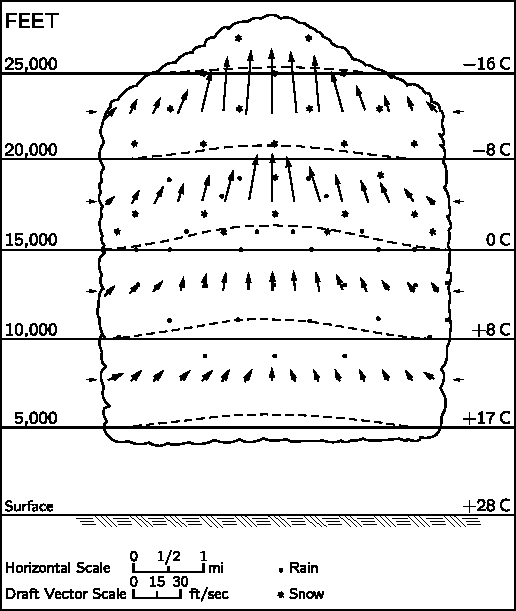
\includegraphics[width=0.6\linewidth]{fyz_fig695.pdf}
      \caption{
               (\cite[s.~707]{Feynman02})}
      \label{fyz:fig695}
    \end{figure}

    \begin{figure}[ht!] %\ref{fyz:fig696}
      \centering
      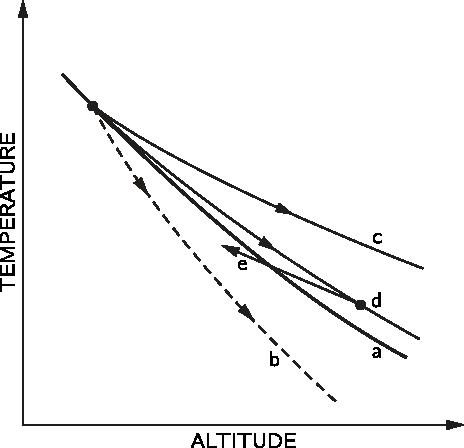
\includegraphics[width=0.6\linewidth]{fyz_fig696.pdf}
      \caption{
               (\cite[s.~707]{Feynman02})}
      \label{fyz:fig696}
    \end{figure}

    \begin{figure}[ht!] %\ref{fyz:fig697}
      \centering
      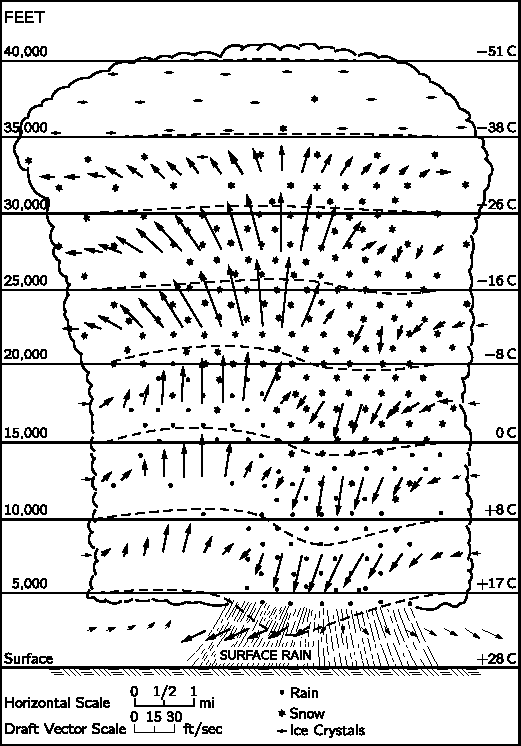
\includegraphics[width=0.6\linewidth]{fyz_fig697.pdf}
      \caption{
               (\cite[s.~707]{Feynman02})}
      \label{fyz:fig697}
    \end{figure}

    \begin{figure}[ht!] %\ref{fyz:fig698}
      \centering
      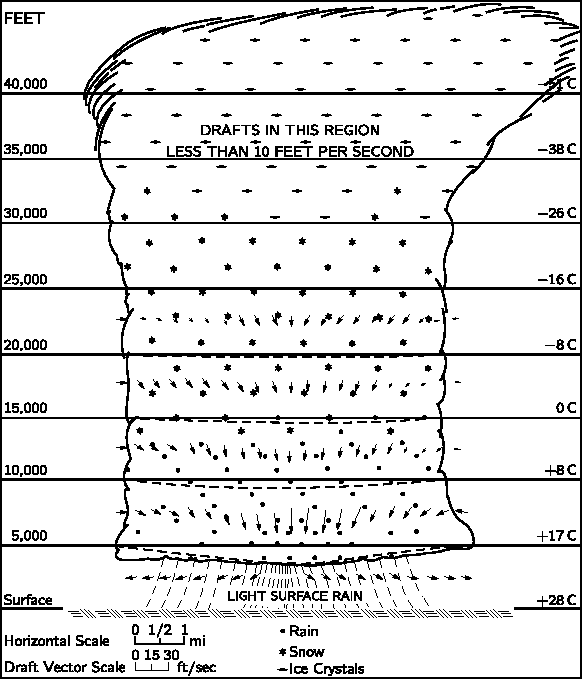
\includegraphics[width=0.6\linewidth]{fyz_fig698.pdf}
      \caption{
               (\cite[s.~707]{Feynman02})}
      \label{fyz:fig698}
    \end{figure}

    \begin{figure}[ht!] %\ref{fyz:fig699}
      \centering
      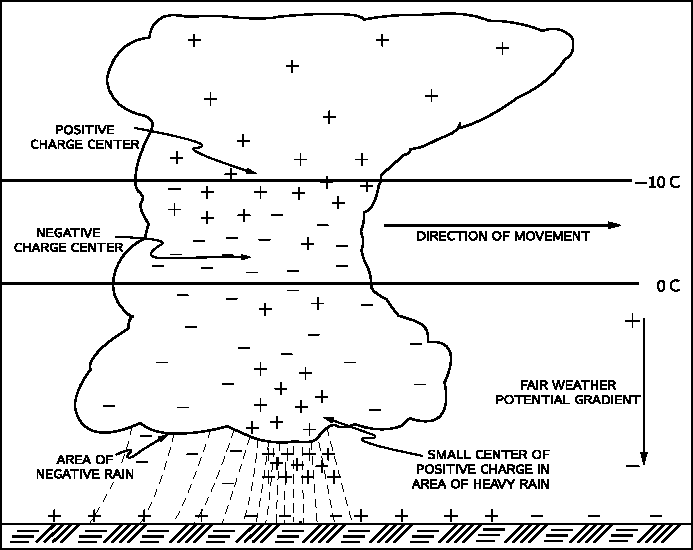
\includegraphics[width=0.6\linewidth]{fyz_fig699.pdf}
      \caption{
               (\cite[s.~707]{Feynman02})}
      \label{fyz:fig699}
    \end{figure}

    \begin{figure}[ht!] %\ref{fyz:fig700}
      \centering
      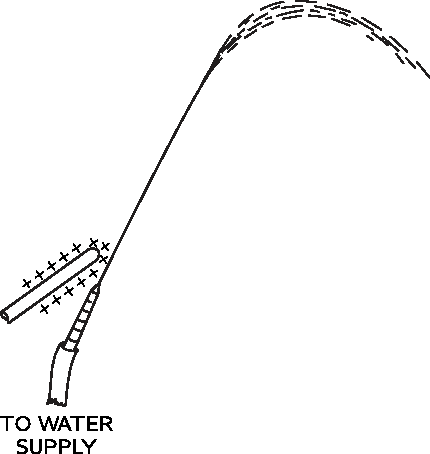
\includegraphics[width=0.6\linewidth]{fyz_fig700.pdf}
      \caption{
               (\cite[s.~707]{Feynman02})}
      \label{fyz:fig700}
    \end{figure}

    \begin{figure}[ht!] %\ref{fyz:fig701}
      \centering
      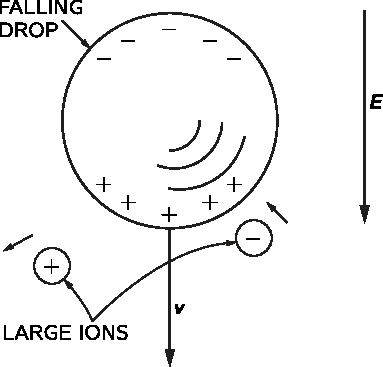
\includegraphics[width=0.6\linewidth]{fyz_fig701.pdf}
      \caption{
               (\cite[s.~707]{Feynman02})}
      \label{fyz:fig701}
    \end{figure}

    \begin{figure}[ht!] %\ref{fyz:fig702}
      \centering
      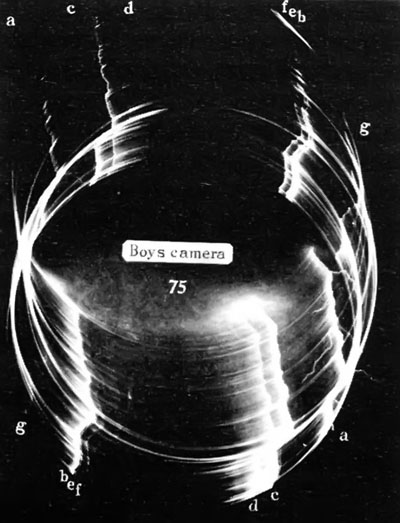
\includegraphics[width=0.6\linewidth]{fyz_fig702.jpg}
      \caption{
               (\cite[s.~707]{Feynman02})}
      \label{fyz:fig702}
    \end{figure}

    \begin{figure}[ht!] %\ref{fyz:fig703}
      \centering
      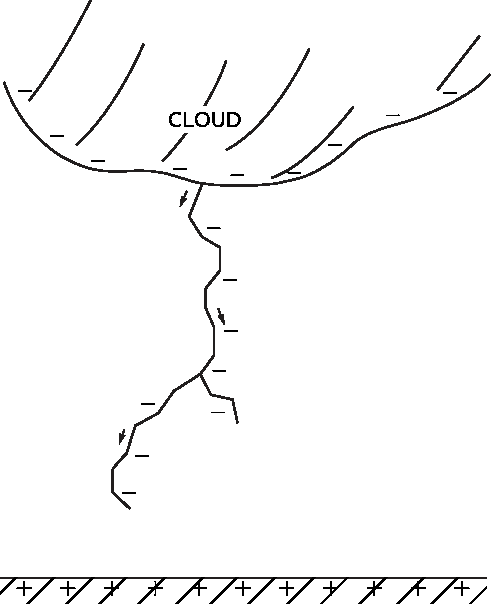
\includegraphics[width=0.6\linewidth]{fyz_fig703.pdf}
      \caption{
               (\cite[s.~707]{Feynman02})}
      \label{fyz:fig703}
    \end{figure}

    \begin{figure}[ht!] %\ref{fyz:fig704}
      \centering
      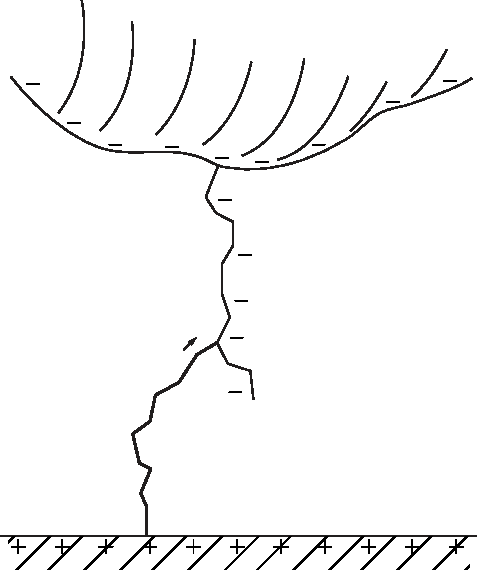
\includegraphics[width=0.6\linewidth]{fyz_fig704.pdf}
      \caption{
               (\cite[s.~707]{Feynman02})}
      \label{fyz:fig704}
    \end{figure}

\todo[inline]{Kapitola fey2ch09 je nedodělaná, obsahuje pouze obrázky}
%} %tikzset
%---------------------------------------------------------------------------------------------------